%%%%%%%%%%%%%%%%%%%%%%%%%%%%%%%%%%%%%%%%%
% The Legrand Orange Book
% LaTeX Template
% Version 1.2 (19/5/13)
%
% This template has been downloaded from:
% http://www.LaTeXTemplates.com
%u
% Original author:
% Mathias Legrand (legrand.mathias@gmail.com)
%
% License:
% CC BY-NC-SA 3.0 (http://creativecommons.org/licenses/by-nc-sa/3.0/)
%
% Compiling this template:
% This template uses biber for its bibliography and makeindex for its index.
% This means that to update the bibliography and index in this template you
% will need to run the following sequence of commands in the template
% directory:
%
% 1) pdflatex main
% 2) makeindex main.idx -s StyleInd.ist
% 3) biber main
% 4) pdflatex main
%
% This template also uses a number of packages which may need to be
% updated to the newest versions for the template to compile. It is strongly
% recommended you update your LaTeX distribution if you have any
% compilation errors.
%
% Important note:
% Chapter heading images should have a 2:1 width:height ratio,
% e.g. 920px width and 460px height.
%
%%%%%%%%%%%%%%%%%%%%%%%%%%%%%%%%%%%%%%%%%

%----------------------------------------------------------------------------------------
%	PACKAGES AND OTHER DOCUMENT CONFIGURATIONS
%----------------------------------------------------------------------------------------

\documentclass[11pt,fleqn]{article} % Default font size and left-justified equations


\usepackage[top=3cm,bottom=3cm,left=3.2cm,right=3.2cm,headsep=10pt,a4paper]{geometry} % Page margins

\usepackage{xcolor} % Required for specifying colors by name
\definecolor{ocre}{RGB}{243,102,25} % Define the orange color used for highlighting throughout the book

% Font Settings
\usepackage{avant} % Use the Avantgarde font for headings
%\usepackage{times} % Use the Times font for headings
\usepackage{microtype} %Slightly tweak font spacing for aesthetics
\usepackage{mathptmx} % Use the Adobe Times Roman as the default text font together with math symbols from the Sym­bol, Chancery and Com­puter Modern fonts
\usepackage[scaled=0.90]{couriers} %What is this used for?

\usepackage{amssymb}
 \usepackage{fancyvrb}
 \usepackage{color}
%define a verbatim text for bold user input
\newcommand\verbbf[1]{\textbf{$\blacksquare$ #1}}
%define a verbatim text without box in front
\newcommand\verbbnbf{\textbf}

\usepackage[pdftitle={Programmers Manual for Developing Bulk Extractor Scanner Plug-ins},
              pdfauthor={Jessica R. Bradley, Simson L. Garfinkel},
              pdfkeywords={bulk extractor, scanners, plug-ins, bulk extractor developers}]{hyperref}

\usepackage{microtype} % Slightly tweak font spacing for aesthetics
%\usepackage[utf8]{inputenc} % Required for including letters with accents
\usepackage[T1]{fontenc} % Use 8-bit encoding that has 256 glyphs


%\usepackage[a4paper,pdftex]{geometry}										% A4paper margins
\setlength{\oddsidemargin}{5mm}												% Remove 'twosided' indentation
\setlength{\evensidemargin}{5mm}

\usepackage[english]{babel}
%\usepackage[protrusion=true,expansion=true]{microtype}	
\usepackage{amsmath,amsfonts,amsthm,amssymb}
\usepackage{graphicx}

\usepackage{tabularx}

%use autoref or Autoref for lowercase or uppercase beginning of references
\usepackage{catoptions}
\makeatletter
\def\figureautorefname{figure}
\def\tableautorefname{table}
\def\Autoref#1{%
  \begingroup
  \edef\reserved@a{\cpttrimspaces{#1}}%
  \ifcsndefTF{r@#1}{%
    \xaftercsname{\expandafter\testreftype\@fourthoffive}
      {r@\reserved@a}.\\{#1}%
  }{%
    \ref{#1}%
  }%
  \endgroup
}
\def\testreftype#1.#2\\#3{%
  \ifcsndefTF{#1autorefname}{%
    \def\reserved@a##1##2\@nil{%
      \uppercase{\def\ref@name{##1}}%
      \csn@edef{#1autorefname}{\ref@name##2}%
      \autoref{#3}%
    }%
    \reserved@a#1\@nil
  }{%
    \autoref{#3}%
  }%
}
\makeatother

\usepackage{amsmath}

\usepackage{booktabs}
\usepackage{makecell}

\usepackage{color}
\usepackage{graphicx}
%\usepackage {hyperref}
\usepackage{listings}
\usepackage{xspace}
\usepackage[toc, page]{appendix}
\usepackage[font=small, labelfont=bf]{caption}
%http://tex.stackexchange.com/questions/27663/using- bold-italic-text-inside-listings

\usepackage{multirow} %for multirow tables


\newcommand{\HRule}{\rule{\linewidth}{0.5mm}}
\usepackage{fancyhdr}

\usepackage{array} 

\raggedbottom

\begin{document}

%define macros for commonly used terms that require special formatting
\newcommand \bulk {\textit{bulk\_extractor}\xspace}
\newcommand \beapi {\textit{be13\_api}\xspace}
\newcommand \mytitle {\emph{bulk\_extractor 1.4}}

\hypersetup{%
    pdfborder = {0 0 0}
}

\lstdefinestyle{customfile}{
basicstyle=\footnotesize, frame=single}

\lstdefinestyle{codelisting}{
basicstyle=\footnotesize\ttfamily,breaklines=true, frame=none} 

\begin{titlepage}

% LaTeX Template: Titlepage
% This is a title page template which be used for both articles and reports.
%
% Copyright: http://www.howtotex.com/
% Date: April 2011
% ------------------------------------------------------------------------------

% -------------------------------------------------------------------------------
% Preamble
% -------------------------------------------------------------------------------
%\documentclass[paper=a4, fontsize=11pt,twoside]{scrartcl}		% KOMA article


% ------------------------------------------------------------------------------
% Definitions (do not change this)
% ------------------------------------------------------------------------------
\newcommand{\TRule}[1]{\rule{\linewidth}{#1}} 	% Horizontal rule

\makeatletter							% Title
\def\printtitle{%						
    {\centering \@title\par}}
\makeatother									

\makeatletter							% Author
\def\printauthor{%					
    {\centering \large \@author}}				
\makeatother							

% ------------------------------------------------------------------------------
% Metadata (Change this)
% ------------------------------------------------------------------------------
\title{	\LARGE \textsc{\mytitle} 	% Subtitle of the document
 \\[1.0cm]													% 2cm spacing
 \TRule{0.5pt} \\										% Upper rule
 \LARGE \textbf{\uppercase{Programmers Manual for Developing Scanner Plug-ins}}	% Title
 \TRule{2pt} \\ [0.5cm]								% Lower rule + 0.5cm spacing
 \normalsize \today									% Todays date
}

\author{
		Authors: \\
		Jessica R. Bradley\\
		Simson L. Garfinkel\\		
}

% ------------------------------------------------------------------------------
% Maketitle
% ------------------------------------------------------------------------------
\thispagestyle{empty}				% Remove page numbering on this page

\printtitle									% Print the title data as defined above
  	\vfill
\printauthor								% Print the author data as defined above














\end{titlepage}


\pagenumbering{roman}
\setlength{\parindent}{0pt} %remove indenting from whole document
\newpage
\tableofcontents
\newpage
\pagenumbering{arabic}

%\renewcommand{\thesection}{\arabic{section}}% define arabic numbering


\section{Introduction}

\subsection{Overview of \bulk}

\bulk is a C++ program that extracts email addresses, credit card numbers, URLs, and other types of information from digital evidence files. \bulk operates on disk images, files or a directory of files and extracts useful information without parsing the file system or file system structures. The input is split into pages and processed by one or more scanners. The results are stored in feature files that can be easily inspected, parsed, or processed with automated tools. \bulk also creates histograms of features that it finds. This is useful because features that are more common tend to be important. \\  

In addition to the capabilities described above, \bulk also includes 
\begin{itemize}	
	\item A BE Viewer User Interface (BEViewer) for browsing features stored in feature files and for launching \bulk scans
	\item A small number of python programs that perform automated processing on feature files
\end{itemize} 
\bulk 1.4 detects and optimistically decompresses data in ZIP, gzip, RAR, and Microsoft's XPress Block Memory Compression algorithm. This has proven useful, for example, for recovering email addresses from within fragments of corrupted system hibernation files. \\

\bulk contains a simple but effective mechanism for protection against decompression bombs. It also has capabilities specifically designed for Windows and malware analysis including decoders for the Windows PE, Linux ELF, VCARD, BASE16 and a Windows directory formats.\\

\bulk gets its speed through the use of compiled search expressions and multi-threading. The search expressions are written as pre-compiled regular expressions, essentially allowing \bulk to perform searches on disparate terms in parallel. Threading is accomplished through the use of an analysis thread pool.  After the features have been extracted, \bulk buildTs a histogram of email addresses, Google search terms, and other extracted features. Stop lists can also be used to remove features not relevant to a case. \\

\bulk is distinguished from other forensic tools by its speed and thoroughness. Because it ignores file system structure, \bulk can process different parts of the disk in parallel. In typical use, the program splits the disk image into 16MiByte pages and processes one page on each available core. This means that 24-core machines processes a disk roughly 24 times faster than a 1-core machine. \bulk is also thorough. It automatically detects, decompresses, and recursively re-processes compressed data that has been compressed with a variety of algorithms. Our testing has shown there is a significant amount of compressed data in the unallocated regions of file systems missed by most forensics tools that are commonly in use today. Another advantage of ignoring file systems is that \bulk can be used to process any digital media. The program has been used to process hard drives, SSDs, optical media, camera cards, cell phones, network packet dumps, and other kinds of digital information.

\subsection{Purpose of this Manual}
This Programmers Manual provides guidelines for \bulk plug-in development. Plug-ins are external scanners that an individual or organization can run in addition to the open source capabilities provided by the tool. The plug-in system gives the full power of \bulk to external developers, as all of \bulk's native scanners are written with the plug-in system. This power gives third party developers the ability to utilize proprietary or protected algorithms in \bulk scanners. \\

This manual is intended for programmers of \bulk scanner plug-ins. It describes an overview of the \bulk architecture demonstrating how the scanners operate, the process for adding a scanner plug-in and guidelines for doing so, and it provides several examples of \bulk scanner plug-ins.

\subsection{Conventions Used in this Manual}
This manual uses standard formatting conventions to highlight variable names, file names, code examples and example commands. The conventions for those specific types are described in this section. \\

File names are displayed in a teletype font. They will appear as \texttt{filename.txt} within the text throughout the manual.\\

Variable and function names are displayed in italics. They appear as \textit{variablename} and \textit{functionname()} within the text throughout the manual.\\

This manual contains example commands that should be typed in by the user. A command entered at the terminal is shown like this: \begin{Verbatim}[commandchars=\\\{\}]
\verbbf{command}
\end{Verbatim}
The first character on the line is the terminal prompt, and should not be typed. The black square is used as the standard prompt in this manual, although the prompt shown on a users screen will vary according to the system they are using.\\

Finally, there are numerous code examples of one line or more throughout the text. Those examples are displayed in a courier font and will be shown as the following: 
\lstset{style=codelisting}
\begin{lstlisting}
	void exampleFunction()
\end{lstlisting}



\section{Setting up Code for Development}


\subsection{How to Get the Code}
There are several ways to obtain the \bulk code base. The recommended way is to download the code in .tar.gz format from the digitalcorpora website at the following url:
\url{http://digitalcorpora.org/downloads/bulk_extractor/} 
This website always has the latest released version. It will be named \textit{bulk\_extractor-(versionnumber)\_(codeversion).tar.gz} where version number will be the number of the code release and code version is the number following the major release number. So, a release for 1.4.0 would be called \textit{bulk\_extractor-1.4.0.tar.gz}. \\

Another way to obtain the development version of the code is to run the git command with the following parameters: 
\begin{Verbatim}[commandchars=\\\{\}]
\verbbf{git clone --recursive https://github.com/simsong/bulk_extractor.git}
\end{Verbatim}

This is intended for \bulk developers only. The code in that location is not considered a stable release. It is almost constantly in development and could be updated or changed at any time. 

\subsection{General Notes on Compiling}
This section includes instructions for compiling \bulk for Linux, Mac and Windows (by cross-compiling on Linux). MacOS and Linux systems provide the easiest and recommended way to compile \bulk but it can be done on Windows systems if necessary.


\subsection{Compiling for MacOS or Linux}

\lstset{basicstyle=\footnotesize\ttfamily,breaklines=true}
If the source is downloaded from github, the next step is to (from the downloaded source directory) run bootstrap.sh, configure and make. If the source is extracted from the .tar.gz file, it is not necessary to run bootstrap.sh. :
\begin{Verbatim}[commandchars=\\\{\}] 
\verbbf{cd bulk_extractor}
\verbbf{sh bootstrap.sh} (only for source obtained from github, not .tar.gz)
\verbbf{sh configure}
\verbbf{make} 
\verbbf{sudo make install}
\end{Verbatim}




\subsection{Compiling for Windows}
The only tested and recommended way to compile for Windows is to cross-compile from a Linux system with MinGW. There are two methods for cross-compiling described below. The primary environment for cross-compiling is Fedora. Fedora is recommended over Ubuntu for several reasons but primarly because the installation is only tested on Fedora. Previous versions compiled natively on Windows using MinGW or cygwin but those methods are currently untested and are not supported at this time.

\subsubsection{Cross-compile for Windows using Fedora}
First, set up the mingw and cross-compilation environment:
\begin{Verbatim}[commandchars=\\\{\}] 
\verbbf{sudo yum -y install mingw64-gcc-c++} 
		         \verbbnbf{mingw64-zlib-static mingw64-pthreads flex}
\verbbf{sudo yum -y install autoconf automake}  (only for source from github)
\verbbf{sudo yum -y install zlib-devel zlib-static}
Run script CONFIGURE_F18.sh found in directory src_win/
\verbbf{make win32}
\verbbf{make win62}
\end{Verbatim}

Next, enable the Windows installer by running configure: 
\begin{Verbatim}[commandchars=\\\{\}] 
\verbbf{./configure --enable-win_installer}
\end{Verbatim}
After enabling the Windows installer, type the following to create the unsigned windows installer. 

\begin{Verbatim}[commandchars=\\\{\}] 
\verbbf{cd win_src && make}
\end{Verbatim}


\subsubsection{Cross-compile for Windows using Debian Testing (wheezy) or Ubuntu 12.04 LTS (with mingw)}
First, you need to install mingw-w64. Go to the directory where you would like to install mingw and run the following command:

\begin{Verbatim}[commandchars=\\\{\}] 
\verbbf{sudo apt-get update}
\verbbf{sudo apt-get upgrade}
\verbbf{sudo apt-get -y install mingw-w64}
\end{Verbatim}
Next, run the following command to allow cross-compiling of the 64-bit and the 32-bit bulk\_extractor.exe (although running the 32-bit version is not recommended).
\begin{Verbatim}[commandchars=\\\{\}] 
\verbbf{./configure --host=i686-w64-mingw32}
\end{Verbatim}


To compile the source, go to the \bulk directory where you ran the git command or extracted the .tar.gz file and run the following commands:
\begin{Verbatim}[commandchars=\\\{\}] 
\verbbf{cd bulk_extractor}
\verbbf{sh bootsrap.sh} (only for source obtained from github, not .tar.gz))
\verbbf{mingw64_configure}
\end{Verbatim}

Using this method, the executables, libraries and scripts required for \bulk are not installed automatically. All of that must be done manually by the user. Again, this is why this method is not recommended or supported.

\subsubsection{Creating a Signed Windows Installer (Optional)}
A certification is not required for the use of \bulk. However, if programmers wish to create a signed installer, the following steps will create a signed Windows installer. Signing tool "osslsigncode" for Authenticode signing of EXE\/CAB files is required. 
\begin{itemize}
\item Install the package \textit{osslsigncode}. 
\item Define and export the Environment variables BE\_CERT and \\
BE\_CERT\_PASSWORD, in order to sign files. 
\item The Environment variable BE\_CERT must be set to the location of the code signing certificate. 
\item The Environment Variable BE\_CERT\_PASSWORD must be set to the password for the code signing certificate.
\end{itemize}
The file \texttt{unistall.exe} must also be present so that it can be signed. Obtaining it requires several steps:

\begin{itemize}
	\item Create the unsigned installer by typing \textit{make} as described above
	\item Run the unsigned installer on a Windows system. This action will additionally install the uninstaller.
	\item Copy the uninstaller from the Windows system back into this directory. It should be at path 
		C:\textbackslash Program Files (x86)\textbackslash Bulk Extractor \textless version\textgreater \textbackslash uninstall.exe 
\end{itemize}

If the system clock on your Windows system is slower, you may need to \textit{touch uninstall.exe} after it is installed in this directory.
Finally, run \textit{make signed} to complete installation.
 \cite{installreadme}

\section{Overview of Architecture}
\bulk is written in C and C++ and uses GNU autotools as a build environment. Development is typically done in Linux or MacOS as described in the previous section.  The key features of the architecture are: 
\begin{itemize}
\item Scanners that look for information of interest in typical investigations
\item Recursive re-analysis of compressed data
\item Results stored in "feature files"
\item Multi-threaded operation
\end{itemize}
This section gives a high level overview of how the architecture works. Later in this document, \textbf{\Autoref{SoftwareDesign}} \textbf{\nameref{SoftwareDesign}} provides the specific implementation details for the key features are discussed in more detail. At a high level, \bulk processes disk images, scans those images and produces feature files. The multi-threaded application runs these steps in parallel on different parts ("pages") of the disk simultaneously. Results are combined by the feature recorder system.\\

Figure ~\ref{fig:systemdiagram} depicts the overall system processing. Thread 0 reads the bulk data into the image processing iterator where the data is divided into sections for processing by the scanners. The application then runs the scanners in multiple threads (threads 1 -- N) to create feature files and histograms of the data found in the images. Scanners each serve a specific purpose, looking for different types of information (email, wordlist) or at different types of data (zip, pdf). The scanners run iteratively, processing data that has been scanned or processed by other scanners.\\


\begin{figure}
	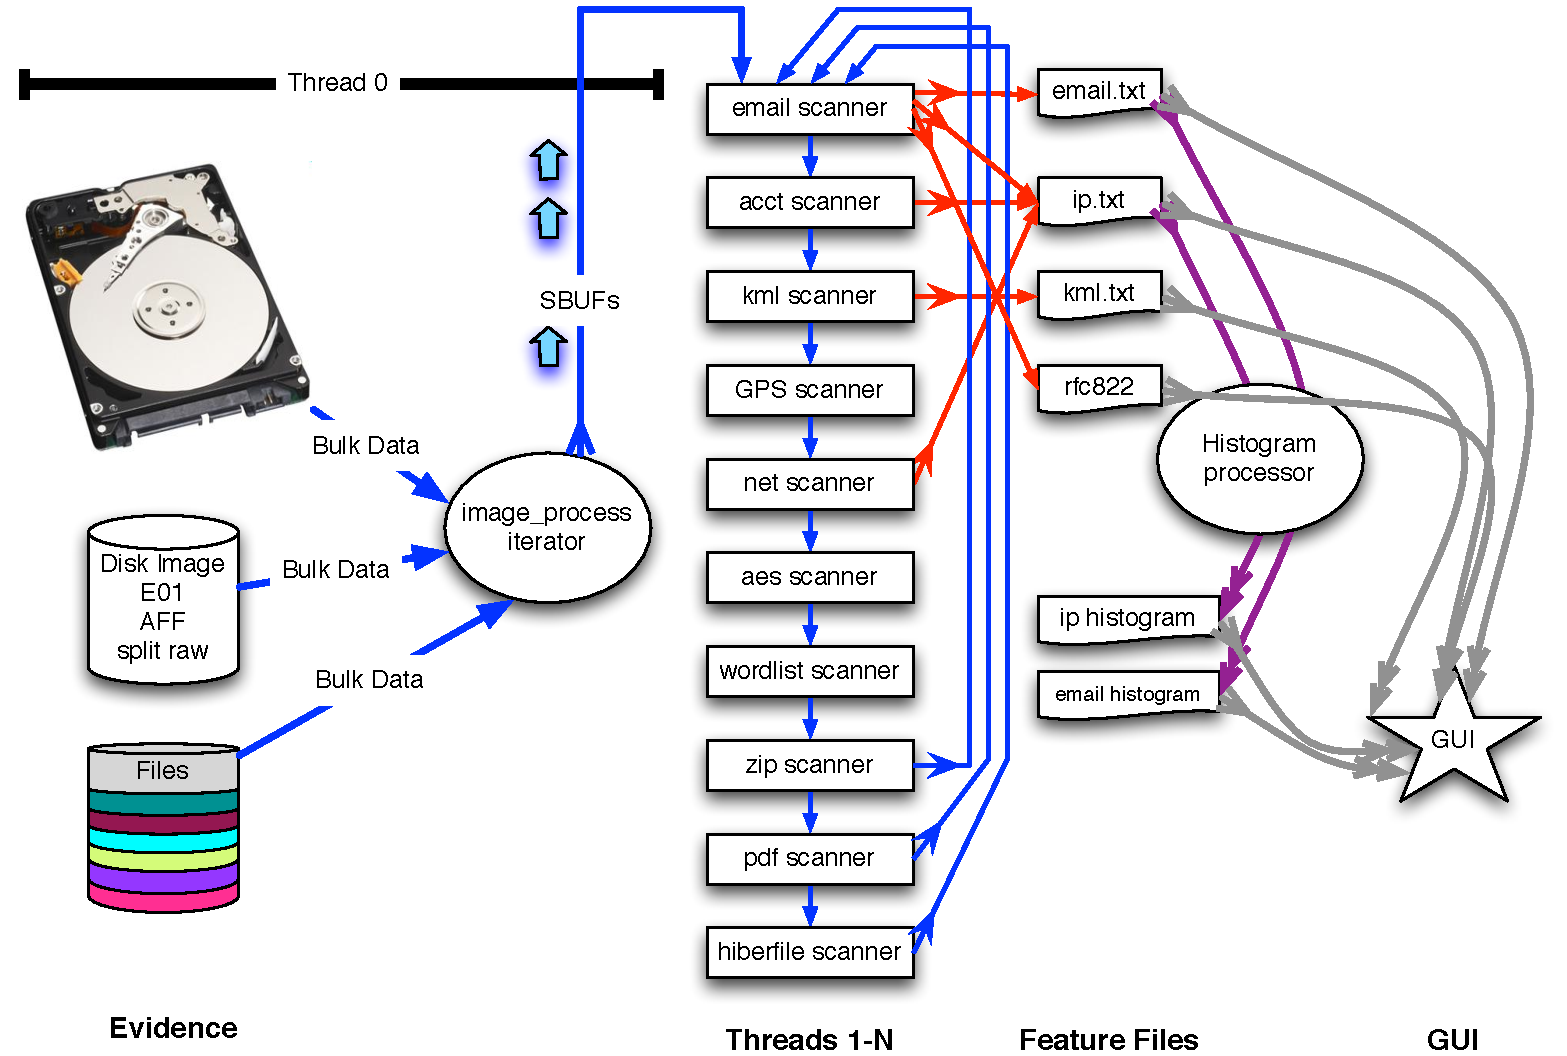
\includegraphics[scale=.50]{system_diagram.pdf}
	\caption{Overall System Architecture of \bulk }
	\label{fig:systemdiagram}
\end{figure}


Image processing handles multiple image formats (including E01, AFF, raw, split raw \&individual disk files), raw devices or files. The image\_process iterator that runs in the first thread (Thread 0) chops the images into sbuf\_t objects (referred to as sbufs). Sbufs ("safer buffer") provide a typesafe means to refer to binary data with the context of \bulk. All data that \bulk processes is divided into sbufs. Sbufs are a block of memory that hold the data, the margin and the path of the first byte (pos0) of a piece of data. The sbuf is typically the size of a page plus a buffer but it can also be smaller or much larger. Pages overlap to avoid dropping features that cross buffer boundaries.  The area of overlap is called the margin.  Each sbuf can be processed in parallel and are not dependent on each other. Features that start in the page but end in the margin are reported. Features that start in the margin are ignored and processed later in a future scanner iteration. The assumption behind the image processing algorithm is that the feature size is smaller than the margin size. A typical margin is 1 MB but it can be made larger with a command line argument. Figure ~\ref{fig:margindepiction} depicts how the \textit{bufsize} overlaps the \textit{pagesize} (difference is the margin - \textit{marginsize}). The disk image is broken into these sbufs for processing. \\

\begin{figure}
	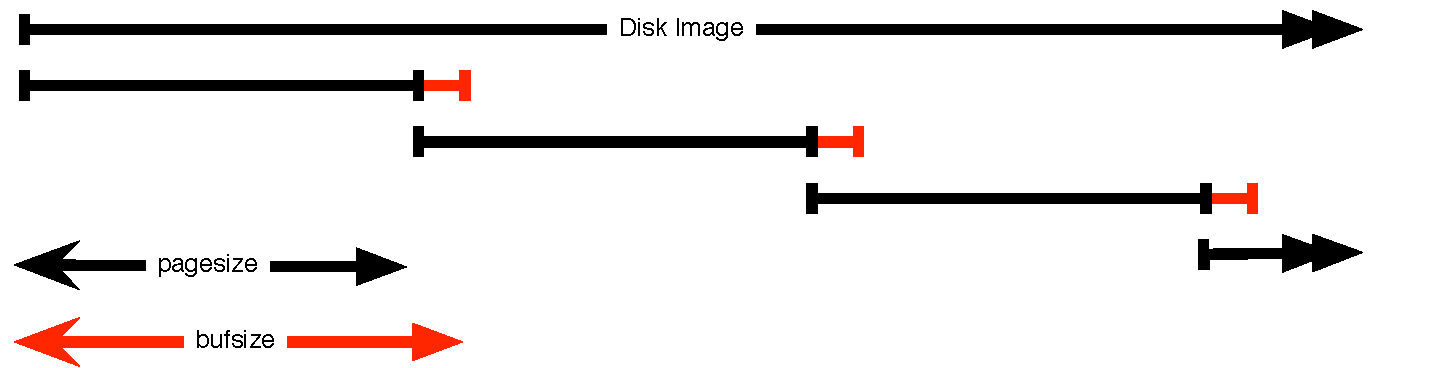
\includegraphics[scale=0.60]{margindepiction.pdf}
	\caption{Image Processor divides the disk image into sbuf objects. Each sbuf object is the size of a page (\textit{pagesize}) with a buffer overlap in an area called the margin (\textit{marginsize} is equal to \textit{bufsize-pagesize}). The sbufs overlap with each other to ensure all information is processed.}
	\label{fig:margindepiction}
\end{figure}


The \textit{image\_process} iterator makes \textit{sbuf\_t} buffers. Each buffer is processed by every enabled scanner. In the \bulk code, \textit{sbuf\_t} objects are described as follows:
\lstset{basicstyle=\footnotesize}

\lstset{style=codelisting}
\begin{lstlisting}
class sbuf_t{
	...
	public:{
	const uint8_t *buf /*data*/
	const pos0_t pos0 /*forensic path*/
	const size_t bufsize
	const size_t pagesize;
...
};
\end{lstlisting}


Scanners process sbufs and extract features.  There are many different types of scanners within \bulk that each look for a different type of information. A given scanner can also be written to discover one or more types of features. For example, the email scanner, as depicted in Figure ~\ref{fig:scannersextractfeatures}, iteratively processes sbuf objects, finds three different types of features and outputs to three feature files including \texttt{email.txt} (includes email addresses), \texttt{rfc822.txt} (includes Message-ID, Date, Subject, Cookie and Host Information) and \texttt{domain.txt} (IP addresses and host names). \\

\begin{figure}
	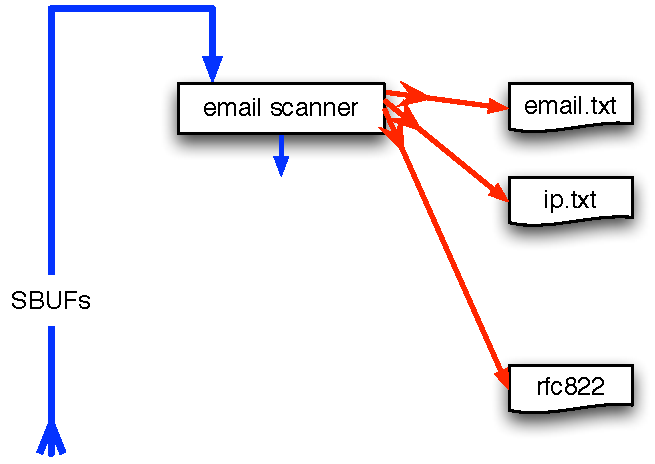
\includegraphics[scale=0.90]{scannersextractfeatures.pdf}
	\caption{The email scanner writes to three different types of feature files.}
	\label{fig:scannersextractfeatures}
\end{figure}

\begin{figure}
	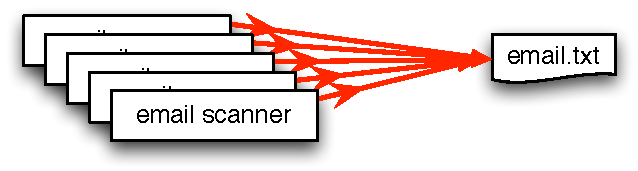
\includegraphics[scale=0.90]{writetoemail.pdf}
	\caption{Many scanners, email scanner among them, will write to the email.txt as email features are discovered during the multi-threaded scanning process.}
	\label{fig:writetoemail}
\end{figure}

Features files are written using the feature recording system. Thread safe feature recorder objects store the features and write the information to the appropriate feature file. Scanners are given a (feature\_recorder *) pointer and as features are discovered, they are sent to the feature recorder. Multiple scanners may have the same feature pointer. As previously stated, the email scanner finds email addresses and those findings are written to email.txt by the feature recorder. Other scanners will find emails throughout scanning that are sent to the email feature recorder and also written to email.txt. Figure ~\ref{fig:writetoemail} shows how many scanners write to one feature file during \bulk scanner operation.\\

A feature files contains rows of features. Each row is typically comprised of an offset, a feature, and the feature in evidence context although scanners are free to store whatever information they wish. A few lines of an email feature file might look like the following:\\ \\

\lstset{style=customfile}
\begin{lstlisting}
OFFSET      FEATURE	        FEATURE IN EVIDENCE CONTEXT
48198832  domexuser2@gmail.com 	__<name>domexuser2@gmail.com/Home
48200361  domexuser2@live.com 	__<name>domexuser2@live.com</name
48413823  siege@preoccupied.net	'Brien  <siege@preoccupied.net>_l
\end{lstlisting}


The types of features displayed in the feature file will vary depending on what type of feature is being stored. However, all feature files use the same format with each row corresponding to one found instance of a feature and three columns describing the related data (offset, feature, and feature in evidence context). Scanner plug-in programmers will have to specify the features that the scanner creates and write to those features during scanning. \\

Histograms are a powerful tool used in \bulk for understanding evidence. A histogram of emails allows us to rapidly determine the drive's primary user, the user's organization, primary correspondents and other email addresses. The feature recording system automatically makes histograms as data is processed. When the scanner writes to the feature recording system, the relevant histograms are automatically updated. Therefore, scanner plug-in programmers will not specifically have to write any information to the histograms. Programmers will only have to specify the type of histogram the scanner creates and subsequent data will be sent to the histograms automatically. \\ 

A histogram file will, in general, look like the following file excerpt:
\lstset{style=customfile}
\begin{lstlisting}
n=875 mozilla@kewis.ch (utf16=3)
n=651 charlie@m57.biz (utf16=120)
n=605 ajbanck@planet.nl
...
n=288 mattwillis@gmail.com
n=281 garths@oeone.com
n=226 michael.buettner@sun.com (utf16=2)
n=225 bugzilla@babylonsounds.com
n=218 berend.cornelius@sun.com
n=210 ips@mail.ips.es
n=201 mschroeder@mozilla.x-home.org
n=186 pat@m57.biz (utf16=1)
\end{lstlisting}
Each line shows a feature and the number of times that feature was found by \bulk. Features are stored in the file in order of occurrence with most frequent features appearing at the top of the file and least frequent displayed at the bottom. \\

\begin{figure}
	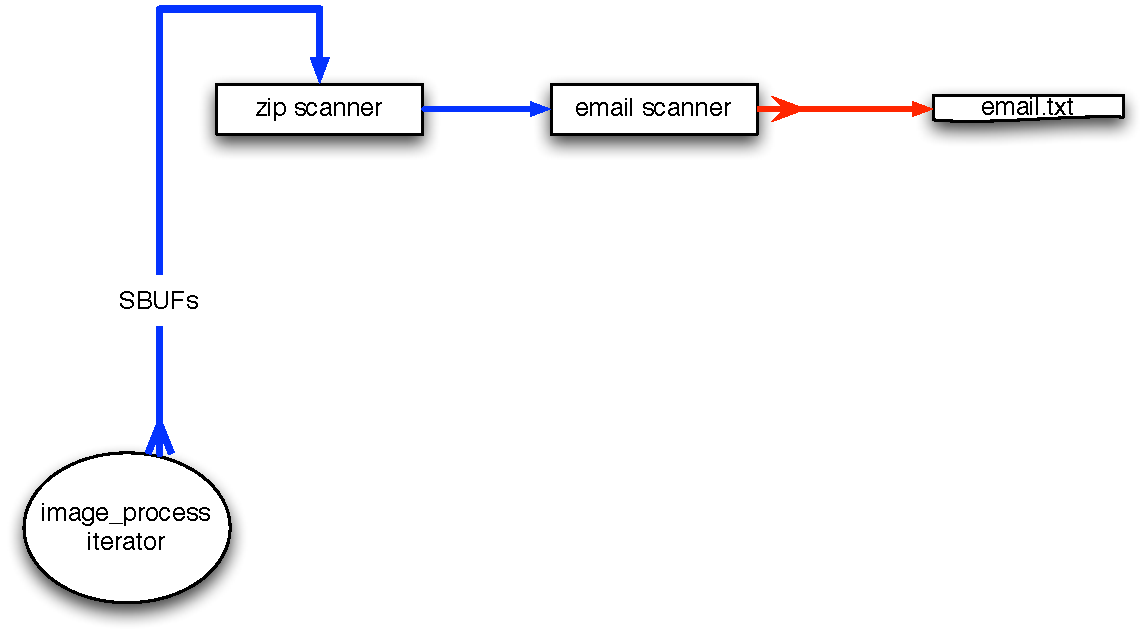
\includegraphics[scale=0.60]{extractinformationreprocess.pdf}
	\caption{To extract a compressed email, sbufs are first decompressed by the zip scanner. Then, decompressed sbuf data is sent to the other scanners (including email scanner). }
	\label{fig:extractinformationreprocess}
\end{figure}

\bulk has multiple scanners that extract features. Each scanner runs in an arbitrary order. Scanners can be enabled or disabled which can be useful for debugging and speed optimization. Some scanners are recursive and actually expand the data they are exploring thereby creating more sbufs. Recursion is used for, among other things, decompressing ZLIB and Windows HIBERFILE, extracting text from PDFs and handling compressed browser cache data. The recursion process requires a new way to describe offsets.\\

\bulk introduces the "forensic path." The forensic path is a description of the origination of a piece of data, whether it be from, for example, a flat file, a data stream, or a decompression of some type of data. Consider an HTTP stream that contains a GZIP-compressed email as shown in Figure ~\ref{fig:extractinformationreprocess}. scan\_zip will find zlib-compressed regions and an sbuf is made for the decompressed data. The data is then re-analyzed by the other scanners. Using this method, \bulk can find email addresses in compressed data.\\

Every forensic tool crashes at times because the tools are routinely used with data fragments, non-standard codings, etc. One major issue is that the evidence that makes the tool crash typically cannot be shared with the developer. The \bulk system implements checkpointing to protect the user and the results. \bulk checkpoints the current page in the file \texttt{report.xml}. After a crash, the user can just hit the up-arrow in the BEViewer and return. \bulk will restart at the next page. \\

The file \texttt{report.xml} is a Digital Forensics XML (DFXML) report that includes information about the source media, how the \bulk program was compiled and run, the time to process the digital evidence, and a meta report of the information that was found. DFXML will be discussed briefly in \textbf{\Autoref{DFXMLSection}} \textbf{\nameref{DFXMLSection}} later in this document. \\

\bulk 's design is integrated but compact. The design allows programmers to implement their own scanners that can be enabled or disabled for different \bulk applications. These scanner plug-ins use the same methodology and code structure as the scanners that are built and distributed with the \bulk system. The methodology to build scanner plug-ins is described in \textbf{\Autoref{WritePlugins}} \textbf{\nameref{WritePlugins}}. The next section provides more details on the specific parts of the \bulk API that are most relevant to scanner plug-in developers. 

\section{Software System Design for Plug-ins}
\label{SoftwareDesign}

The module \beapi is the API for \bulk. It provides the software description and implementation for sbufs, feature recorders and the complete scanner plug-in system API. The \beapi module is located inside the /src directory. Histograms are also described and implemented in the /src directory. \\

The \textit{dfxml} module, also located in the /src directory, provides capabilities that may be useful to scanner plug-in programmers. The \textit{dfxml}  module defines and implements the Digital Forensics XML (DFXML) language, enabling the exchange of structured forensic information for \bulk. Both the \beapi and the \textit{dfxml} modules are standalone git modules and can be obtained separately using the git command. To obtain the \beapi module, run the following command from the directory where you want to install it:
\begin{Verbatim}[commandchars=\\\{\}]
\verbbf{git clone --recursive  https://github.com/simsong/be13_api.git}
\end{Verbatim}
To obtain the \textit{dfxml} module, run the following command from the directory where you want to install it:
\begin{Verbatim}[commandchars=\\\{\}]
\verbbf{git clone --recursive https://github.com/simsong/dfxml.git}
\end{Verbatim}
It is not necessary to install these modules separately if you have already installed the \bulk code. Both of these modules are downloaded as part of the \bulk code installation described earlier in this manual. \\


The following sections describe the capabilities and relevant implementation details found in \beapi, \textit{dfxml} and the \texttt{histogram.h} file. Specific implementation and usage information details can be found in the directories and .h files referenced below. 

\subsection{be13\_api Module}
The \beapi module is the API for \bulk version 1.3 and 1.4. The API was introduced with \bulk version 1.3. \bulk modules must be recompiled for each version of the program but no source code changes should be required. The most important and relevant information in the module for scanner plug-in programmers is that which describes sbufs, feature recorders and the plug-in system API.

\subsubsection{Sbufs}
Sbufs ("safer buffer") provide a typesafe means to refer to binary data with the context of \bulk. As previously stated, all data that \bulk processes is divided into sbufs. Those sbufs are then processed by all enabled scanners. The sbuf processed by a scanner may originate from a disk, a disk image or be the result of decompressing or otherwise decoding other data (note: recursive scanners that decompress or decode data will produce sbufs that will then be processed by other scanners). For the complete listing of sbuf data and functions, see \texttt{sbuf.h} in the \beapi directory.\\

\textbf{Sbuf Data} \\
Sbufs are a block of memory that hold the data, the margin and the forensic path of the first byte (pos0) of a piece of data. Specifically, the most relevant public member variables are: 
\begin{itemize}
\item \textit{bufsize} - (size\_t) the size of the buffer
\item \textit{pagedata}  - (size\_t) page data (margin size is not explicitly stored because it is equal to bufsize - pagesize) 
\item \textit{pos0} - (pos0\_t) the path of the first byte 
\end{itemize}

\textbf{pos0} \\
The pos0 variable is not simply the "start of the buffer." It refers more generally to the address of the first byte because the sbuf could be the result of a transformation (decompression or decoding).The pos0 actually holds a string to the base path and the offset into that path.  In that case, the sbuf can include string associated with decompressors and ordinals associated with offsets. For example, 1000-GZIP-300-BASE64-30 means go 1000 bytes into the stream, unzip, go 300 bytes into the decompressed stream, un-BASE64, and go 30 bytes into that. This is not always the case. Simpler sbufs will use pos0 to hold the address of the start of the buffer, but the capability for a more complex representation is available and often used. The pos0 class is also defined in \texttt{sbuf.h}.\\

pos0 functions useful to scanner plug-in programmers include:
\begin{itemize}
\item \textit{bool isRecursive()} - a function to determine if it's recursive
\item \textit{pos0\_t shift()} (int64\_t s) - function to return a new position that's been shifted by an offset
\item \textit{std::string firstPart()} function to return the first part of the pos0, \textit{std::string lastAddedPart()} function to return the last added part of the pos0, and \textit{std::string alphaPart()} function to return the non-numeric part of the pos0 
\item Comparison operations that compare two pos0's including >, < and ==
\end{itemize}

\textbf{Important Sbuf Properties and Functions} \\
There are several ways to allocate an sbuf including mapping from a file, setting from a block of memory and creating a subset of an existing sbuf. The \textit{sbuf\_t} class remembers how the sbuf was allocated and automatically frees whatever resources are needed when it is freed. Scanner plug-in programmers must be careful when deleting sbuf structures. They must be deleted in First-in, Last-out order or memory can be corrupted. For example, if you create an sbuf from a mapped file, you must first delete the sbuf before unmapping the file or the subset sbuf will point to unallocated memory. \\

Table ~\ref{tab:SbufFunctions} describes the most important sbuf functions that can be utilized by scanner plug-in programmers as needed. Also refer to \texttt{sbuf.h} for all of the sbuf member variable and function information.

\newcolumntype{V}{>{\centering\arraybackslash} m{4 cm} }

\begin{table}[!ht]
\centering
\caption{Sbuf Functions}
\label{tab:SbufFunctions}
%\begin{tabular}{|V|m{8cm}|}
%\resizebox{30cm}{!}{
\begin{tabular}{|c|m{8cm}|}
\hline \hline
\textbf{Function Grouping} & \textbf{Functions Available} \\
\hline
\multirow{6}{4 cm}{\centering \newline \newline \newline \newline \newline \newline Creating an Sbuf} & Create from a parent (with the same or different path) \\\cline{2-2}
 & Allocate with a position but no data (used when an sbuf needs to be passed but has no data)  \\\cline{2-2}
 & Allocate from an existing buffer (optionally freeing that buffer)\\\cline{2-2} 
& Allocate from an existing sbuf where the allocated sbuf MUST be freed before the source because no copy is actually made\\\cline{2-2}
& Use + operator on sbuf + i bytes, returns a new sbuf that is i bytes into the original sbuf. New sbuf is a child. If parent gets deleted then child points to invalid memory \\\cline{2-2}
& Allocate an sbuf from a file mapped into memory \textit{static sbuf\_t *map\_file(...)} \\\cline{2-2}
\hline
\multirow{2}{4 cm}{\centering \newline Parent-Child Information}  & Get the parent of the parent (\textit{const sbuf\_t *highestparent() const}) \\\cline{2-2}
& Add (\textit{void add\_child(const sbuf\_t \& child) const}) and delete (\textit{void del\_child(const sbuf\_t \&child) const)}) children\\\cline{2-2}
\hline
\multirow{3}{4 cm}{\centering Helper Functions \& Public Variables} & Deleting sbuf - keep track of whether or not to unmap (\textit{bool should\_unmap}) or free the buffer (\textit{bool should\_free}) and close the fd (\textit{bool should\_close}) when the sbuf is deleted \\\cline{2-2}
& Find offset of a byte (\textit{size\_t offset(const uint8\_t *loc)}) \\\cline{2-2}
& Return the sbuf as a String (\textit{std::string asString()}) \\\cline{2-2}
\hline
\multirow{8}{4 cm}{\centering \newline \newline \newline \newline \newline \newline \newline \newline \newline Integer \& String Type Ops} & memcmp search functions at a particular location (\textit{int memcmp(const uint8\_t *cbuf,size\_t at,size\_t len)}) \\\cline{2-2} 
&  Return various signed (ex. - \textit{int64\_t get64i(size\_t i) const}) or unsigned (ex. - \textit{uint8\_t  get8u(size\_t i) const}) integer value for the offset of i in Intel (little-Endian) byte order\\\cline{2-2} 
& Return signed (ex. - \textit{int32\_t get32iBE(size\_t i) const}) or unsigned (ex. - \textit{uint16\_t get16uBE(size\_t i) const}) integer value for the offset of i in Motorola (big-Endian byte order) \\\cline{2-2} 
& Functions to get signed (ex. -\textit{int16\_t get16i(size\_t i,byte\_order\_t bo) const})  and unsigned (ex. - \textit{uint8\_t  get8u(size\_t i,byte\_order\_t bo) const}) integers and specify the byte order as input \\\cline{2-2} 
& String readers (\textit{void getUTF8WithQuoting(...)}) \\\cline{2-2}
& [] operator to return what is at index [i]\\\cline{2-2} 
& Find the next occurence of a character or char* in the buffer starting at a given point (\textit{ssize\_t find(uint8\_t ch, size\_t start}) const) \\\cline{2-2} 
& Make a substring (\textit{std::string substr(...)}) \\\cline{2-2}
\hline
\end{tabular}
%}
\end{table}





\subsubsection{Feature Recorders}
Feature recorders are used to record the features found by \bulk scanners and to perform the histogram calculation. There is one \textit{feature\_recorder} pointer per feature file.  Feature recorders will automatically also check the global \textit{alert\_list} to see if the feature should be written to the alert file. They also work with the global \textit{stop\_list}, finding features that are not written to any specific feature file but are written to a \textit{stop\_list} instead.\\

Each scanner will use one or more feature recorders to write the features that if finds to feature files. Scanner plug-in programmers will only use the virtual functions defined in \texttt{feature\_recorder.h}. The virtual functions are all thread safe.   Plug-in programmers can set feature recorder flags including flags that disable the recorder,  refrain from writing the feature's context, ignore the stoplist, ignore the alertlist, disable quoting of non-UTF8 characters in feature files, and  send UTF-8 XML.\\  

To write to the feature recorder system, the programmer can call any of the following \textit{feature\_recorder} virtual methods:

\lstset{style=codelisting}
 \begin{lstlisting}
printf(const char *fmt_, ...) _attribute_((format(printf, 2, 3)));
write(const pos0_t & pos0, 
	const string & feature, const string & context);
write_buf(const sbuf_t & sbuf, size_t pos, size_t len); 
\end{lstlisting}
\textit{printf()} prints to the feature file with no specified format. This function can be used for adding comments to the feature file. \textit{write()} writes the location of a feature, the feature, and its context (the feature may be in the context but it does not need to be). \textit{write\_buf()} writes a feature located at a given place within an sbuf and the context is written automatically. \textit{write\_buf()} provides programmers with the easiest way to write to the feature file. It automatically writes everything, escaping bytes as necessary.\\
 
Feature recorders also provide support for carving (including encoded JPEG carving).   Specifically, the feature recorder stores a set of strings, called \textit{carved\_set}. This is a set of hex hash values of objects that have been carved. There is also a file number and file extension. The \textit{int64\_t file\_number} starts at zero and gets incremented by the carve function. The \textit{string file\_extension} includes '.' and must be set by the caller. The carve function (\textit{virtual void carve(const sbuf\_t \&sbuf,size\_t pos,size\_t len,const struct be13::hash\_def \&hasher}) writes the filename to the feature file where the context is the file's hash using the provided hash function. Carving automatically de-duplicates.
\\

\textbf{Histograms} \\
Histograms are automatically created by feature recorders. Scanner plug-in programmers need only indicate the name of the histograms (\textit{histogram\_defs}) created by their scanner. Histogram names typically correspond to the root name of the feature file.  They will be grouped in those files accordingly. For example, if the scanner plug-in finds email addresses, the programmer would indicate "email" as one of the types of features found by the scanner. As the scanner finds email addresses, those features will be recorded and grouped according to the indicated histogram type ("email"). The histograms that are created can be used to examine the output of \bulk runs.  They demonstrate the frequency of a given feature as it was found in the data and are grouped by data type. 


\subsubsection{Plug-in API}
The complete plug-in API is specified in the file \texttt{bulk\_extractor\_i.h} found in the \beapi directory. It is the only file that must be included in all plug-in source code. The plug-in is implemented as a single function called with two arguments. The plug-in API describes two major components that are important for scanners. The first is the \textit{scanner\_params} which provides mechanisms to pass information to the scanner from the API and from the API to the scanner. The second is the \textit{recursion\_control\_block} which provides important callback information for all recursive scanners. \\

Plug-ins can be linked directly into \bulk and turned into shared libraries within the \bulk system. In order to do that, they should be placed in the same directory as the other scanner executables, /src above the \beapi directory. If they are linked in, they must be referenced in \texttt{bulk\_extractor.cpp}.\\

\textbf{Scanner Params}\\
\textit{scanner\_params} are used primarily to pass information from the api to the scanner. The information passed through them includes the version number, the current phase (discussed later in this section), the sbuf to be scanned and \textit{scanner\_info} (used to pass information from the scanner to the API, also discussed later in this section). Table ~\ref{tab:ScannerParams} describes some of the specific components of \textit{scanner\_params} most relevant to scanner plug-in programmers. \\

\begin{table}[ht]
\centering
\caption{Important Scanner Params}
\label{tab:ScannerParams}
\begin{tabular}{|p{2 cm}|p{3 cm}|p{9 cm}|}
\hline \hline
\textbf{Name} & \textbf{Type} & \textbf{Parameter Purpose} \\
\hline
sp\_version  & int & version number of this structure \\
\hline
phase & phase\_t & denotes the current phase of the scanner \\
\hline
sbuf & sbuf & buffer to scan - only relevant in PHASE\_SCAN \\
\hline
fs & feature\_recorder & feature recorder used to store results of scan \\
\hline
depth & uint32\_t & depth of scan (how far down are we?) \\
\hline
info & scanner\_info & scanner information sent from scanner to API \\
\hline
\end{tabular}
\end{table}

\textbf{Phases - part of the scanner\_params}
The scanner plug-in is called in phases.   The five distinct phases are defined using an enumerated type. Scanners do not have to perform actions in each phase but scanner programmers are able to utilize those phases as required. Currently defined phases for plug-ins are:

\begin{itemize}
	\item PHASE\_STARTUP - called in main thread when scanner loads, called for every scanner
	\item PHASE\_INIT - called in main thread for every ENABLED scanner after all scanners are loaded
	\item PHASE\_THREAD\_BEFORE\_SCAN - called in worker thread for every ENABLED scanner before first scan
	\item PHASE\_SCAN  - called in worker thread for ever ENABLED scanner to scan an sbuf
	\item PHASE\_SHUTDOWN - called in main thread for every ENABLED scanner when scanner is shutdown
\end{itemize}

There are specific actions that should be performed in each phase depending on the desired capabilties of the scanner. Guidelines for scanner plug-in development in each phase can be found in the \nameref{GuidelinesforDevelopment} section.\\

\textbf{scanner\_info - part of the scanner\_params:}
The \textit{scanner\_param} variable, \textit{scanner\_info}, allows the scanner to pass information about itself to the API at startup.  The types of parameters that the scanner sets include name, author, feature file and histogram information.  Through the \textit{scanner\_info} variable the programmer can set the parameters defined in Table ~\ref{tab:scannerinfotoset}. Of note, there is a also a parameter \textit{get\_config} used to get information from the API. That is described in the next section. 
\begin{table}[!ht]

\centering
\caption{scanner\_info Information to Set}
\label{tab:scannerinfotoset}
\begin{tabular}{|p{3 cm}|p{3cm}|p{7 cm}|}
\hline \hline
\textbf{Name} & \textbf{Type} & \textbf{Parameter Definition} \\
\hline
si\_version & int & version number for this structure \\
\hline
name & string & scanner name \\
\hline
author & string & author of the scanner \\
\hline
description & string & description of what the scanner does \\
\hline
url & string & where the scanner came from \\
\hline
scanner\_version & string & version of this scanner\\
\hline
flags & uint64\_t & flags \\
\hline
feature\_names & set<string> & features this scanner needs - used to create feature files\\
\hline
histogram\_defs & histograms\_t & histogram definition information - used to run regex on a feature file and automatically create a histogram \\
\hline
\end{tabular}
\end{table}

Flags are used by the scanner to signal information about themselves to the plug-in system. Programmers can use these flags to tell the API specific things about the scanner. The flags that can be set include: 
\begin{itemize}
\item SCANNER\_DISABLED - scanners are enabled by default unless this is set
\item SCANNER\_NO\_USAGE - indicates the scanner will not show up in the usage statement (can be used to make a 
scanner "hidden" from \bulk users)
\item SCANNER\_NO\_ALL - indicates the scanner won't be automatically enabled when users "enable all" - it must be explicitly declared enabled to run
\item SCANNER\_FIND\_SCANNER - indicates the scanner will use the find list
\item SCANNER\_RECURSE - indicates the scanner will recurse
\item SCANNER\_RECURSE\_EXPAND - indicates the recursive scanner will expand the data (such as a zip scanner that unzips the data)
\item SCANNER\_WANTS\_NGRAMS - indicates this scanner wants constant data (the types of data on disks filled with null or repeating "blank" text such as ABABAB, etc) - without this flag set, scanners will not be called for sbufs containing just repeating ngrams
\item SCANNER\_FAST\_FIND - indicates this scanner is self designating as a scanner that implements -f but is declaring itself faster than other find scanners  
\end{itemize}

\textbf{scanner\_config - part of the scanner\_info:}
The \textit{scanner\_config}, part of the \textit{scanner\_info} variable, is used by the plug-in programmer to get information from the API about or useful to the scanner. It includes the name vals array and access to the global debug variable (programmers don't have to extern it). It also includes the \textit{hash\_def}.  A lot of scanners need to compute cryptographic hashes. The \textit{hash\_def} variable allows the \bulk user to specify which hash algorithm will be used by the scanner. For example, some users might prefer sha1 hashing over MD5. The \textit{hash\_def} defines a name and callback function to indicate a specific hashing function. In the \textit{scanner\_config}, the hashing function is simply passed into the scanner via the \textit{hash\_def}. The programmer does not need to know which function will be performing the hashing, only that it should use the \textit{hash\_def} reference. \\ 

\textbf{Recursion Control Block} \\
The other aspect of the \beapi relevant to scanner plug-in programmers building recursive scanners is the \textit{recursion\_control\_block}. While it is only relevant for recursive scanners, the parameter is passed in to all scanners as one of the two input parameters (along with \textit{scanner\_params}). Recursive scanners should be thread safe and exception safe.  Scanners do not need to test and return after calling the \textit{recursion\_control\_block}, it will simply throw an exception when it finishes its work. The recursion control information includes the public variables indicated in Table ~\ref{tab:RecursionControlBlockParams}. 
\begin{table}[ht]

\centering
\caption{Recursion Control Block Parameters}
\label{tab:RecursionControlBlockParams}
\begin{tabular}{|p{3 cm}|p{2 cm}|p{7 cm}|}
\hline \hline
\textbf{Name} & \textbf{Type} & \textbf{Parameter Purpose} \\
\hline
callback\_  & process\_t & the function to call back \\
\hline
partName\_ & string & the part of the forensic path processed by this scanner \\
\hline
\end{tabular}
\end{table}

An example of a recursive scanner plug-in can be found later in this document in \textbf{Section 5.4.2} \textbf{\nameref{XORScanner}}. It illustrates the usage of the \textit{recursion\_control\_block} variables.


\subsection{DFXML}
\label{DFXMLSection}
Digital Forensics XML (DFXML) is an XML language designed to represent a wide range of forensic information and forensic processing results. It allows the sharing of structured information between independent tools and organizations. \bulk can both emit and consume DFXML \cite{dfxmlpaper}. The DFXML module in \bulk includes capabilities to describe common forensic processes (specifically, cryptographic hashes for md5, sha1, and sha256), forensic work products (such as the location of files on a hard drive) and metadata (such as filenames and timestamps). While the \bulk program uses DFXML as an important part of the input and output processes, including some python scripts, it is not heavily used within the scanners. As previously mentioned in this document, \texttt{report.xml} is generated by \bulk using DFXML and captures infomration about the provenance of the \bulk run.

\section{Writing a Scanner Plug-in}
\label{WritePlugins}
\subsection{Creating a Plug-in Shared Library}
\bulk scanner plug-ins are implemented as shared libraries that begin with the name "scan\_". For example, the demo plug-in that counts the number of blank sectors and prints a report of the percentage of the disk that is blank is called \textit{scan\_blank.so} on Linux and Mac and \textit{scan\_blank.DLL} on Windows. \\

When \bulk begins, it examines the plug-ins directory for all of the shared libraries whose name begins "scan\_". Each one is loaded into the address space. \bulk scanner plug-ins are written in C++ but are called with C linkage to avoid name mangling issues. The plug-in interface is a single C++ function with the same name as the shared library.  For example, for a scanner plug-in named \textit{scan\_sample}:
\lstset{style=codelisting}
\begin{lstlisting}
   extern "C" 
   void scan_sample(const class scanner_params &sp,
              const class recursion_control_block &rcb);

\end{lstlisting}

The plug-in takes two arguments, both of which are references to C++ objects.  The first parameter (\textit{scanner\_params}) provides the general parameters required by the scanner and provides a mechanism for sending the scanner parameters that pertain to the sbuf to be scanned. The second scanner function parameter (\textit{recursion\_control\_block}) is the recursion control block, which provides information for use by recursive scanners (e.g. scanners that perform some kind of transformation on the data and then request re-analysis). It keeps track of the callback function and the forensic path processed by the scanner. \\ 

The file \texttt{bulk\_extractor\_i.h} contains the \bulk plug-in interface. It is the only file that is required by the \bulk system for plug-ins. By design this file contains the minimum necessary for a functional plug-in. This approach minimizes possible interactions between the \bulk system and the plug-in system.


\subsection{Packaging}

The scanner should ideally consist of a single .cpp file called \texttt{scan\_xyz.cpp} where xyz is some description of the type of features extracted by the scanner). There really is no need for a .h file. If the
scanner will be linked in to \bulk then the scanner name must be put at the end of the \texttt{bulk\_extractor.h} file. \\

If there is a need for unicode support, then the scanner should include
should  \textit{\#include "utf8.h" }to use the excellent GNU UTF-8 support package.

\subsection{Guidelines for Development}
\label{GuidelinesforDevelopment}
There are guidelines that can assist the scanner plug-in developer to create safe and efficient code for all of the scanner's phases. The startup, init and shutdown phases are run from the main thread while the thread-before-scan and scan phases are run in multiple threads simultaneously. The multi-threaded \bulk architecture allows programmers to write code that executes in a multi-threaded environment with little effort. Programmers do not need mutexes, spin-locks, pthreads, synchronization elements, or any other traditional threading mechanisms in their code for the multi-threaded phases. Instead, bulk handles this as part of the workload dispatch system. \\ 

Programmers must be vigilant that code \emph{is} running in a multi-threaded environment. Plug-ins MUST BE THREAD SAFE. This can not be emphasized enough. Multiple copies of the code may be running at the same time and accessing the same global
variables. Many programming practices that are acceptable in a single-threaded environment will generate unexpected crashes in a multi-threaded environment. The good news is that these are generally not very good programming practices, so they shouldn't be used anyway. \\

For more information on debugging \bulk scanners, refer to the documentation created by Simson Garfinkel titled \texttt{be\_crash\_diagnostics}. It can be found in the github repository at the following url: \url{https://github.com/simsong/bulk_extractor/blob/master/doc/Diagnostics_Notes/be_crash_diagnostics} \\

In general, here is what happens from a threading perspective when the scanner runs and a few simple rules to follow for each of the phases.

\subsubsection{PHASE\_STARTUP}

The scanner will be called in the startup phase only once. The scanner is called from the main thread for all scanners when the scanner loads (whether or not the scanner is ENABLED).  This phase should be used to load the scanner, get/set metadata and quit. This is, in particular, because disabled scanners will go through this phase and there is no reason to perform any kind of expensive operations on disabled scanners. \textit{scanner\_params} can be used to access any required \textit{scanner\_info} and configuration information that is useful for all (enabled or disabled) scanners.

\subsubsection{PHASE\_INIT}
During this phase the enabled scanner should initialize any global variables that it needs to access. These variables should be \emph{static} so that there is no possibility that they will impact other scanners. Because this is only called from main thread for enabled scanners, this phase can be used to perform more expensive operations that need to be performed. 

\subsubsection{PHASE\_THREAD\_BEFORE\_SCAN}
If an enabled scanner requires thread local storage, the thread specific initialization should be done here. For example, if the scanner needed a socket to a program that isn't multi-threaded (such as a python bridge), this operation would be performed for every thread in this phase.

\subsubsection{PHASE\_SCAN}
The enabled scanner will be called in the scan phase for every page that is processed. The scanner may also be called by multiple threads simultaneously. The chance that multiple threads will be in the scanner simultaneously increasingly linearly with the amount of CPU load that the scanner creates, for the simple reason that the scanner is consuming a larger fraction of all the scanner time.\\ 

Scanners can be tested by running them as the \emph{only} scanner. To do this, use the \emph{-E scanner} option, which
enables \emph{scanner} and disables all of the others. The scanner will be called a LOT. For processing a 1TB drive image,
the scanner will be called at least \(\frac{1,000,000,000,000}{16,777,216} = 59,604\) times.  The scanner will also be called every time \bulk recursively processes a block of data. In a typical run against a 1TB drive image, assume that the scanner will be called at least 500,000 times on data segments ranging from 16MiB to 4096 bytes in size.\\

Each time the scanner is called in the scan phase, it will process one sbuf (accessed through the \textit{scanner\_params sp} variable). The scanner should process that sbuf and, in general, keep all of its per-thread state on the stack. Any global variable that the scanner accesses \emph{should only be accessed with const pointers}. This cannot be stressed enough. More on the specifics of programming with const pointers can be found in the \nameref{StyleGuide} section of this document. \\

All items that the scanner saves should be saved using the \bulk feature recorder system. All of the exposed virtual methods methods are guaranteed to be thread-safe. \\

If for some reason the scanner requires access to a global variable, use
\textit{\_\_sync\_fetch\_and\_add()}. For example, the following function increments \textit{counter} by 1 and
executes the function bar\(\) if the value of \textit{\_sync\_fetch\_and\_add()} is equal to 10:

\lstset{style=codelisting}
\begin{lstlisting}
   if(__sync_fetch_and_add(&counter,1)==10){
     bar();
   }
\end{lstlisting}

If you want to test the value of counter without incrementing it, use
this:
\begin{lstlisting}
   if(__sync_fetch_and_add(&counter,0)==10){
     bar();
   }
\end{lstlisting}

The programmer must remember that \emph{once a global variable is modified in a multi-threaded environment, you may only access that variable using thread-aware code.} That is because the thread-aware code will use the correct barriers, mutexes or locks necessary on the system's architecture to get a current copy of the global variable. This is especially important on systems with multiple processes and multiple caches. \textit{\_\_sync\_fetch\_and\_add()} is a GCC built-in. A full memory barrier is created when this function is invoked.\\

For complex data types, there may be instances where corrupt features are found when some, but not all, of the feature is valid. In that case, the scanner should be designed to accept data until an invalid size or offset is encountered, at which point what is accumulated so far is reported. \\

In the case of the Exchangeable Image File Format (EXIF), for example, it is hard to get a false positive.  First, the 4-byte EXIF magic number is found. After that the the 4-byte Endian and magic number signature must be present.  Then the scanner must search through valid 2-byte application markers until the APP1 jpeg marker is found. Finally, the 6-byte Tiff signature must be present ("Exif\textbackslash 0\textbackslash 0"). When this signature is found, the scanner accepts the feature. As with any feature, it is possible for some of the information to be corrupted because it is part of an overwritten sector. The data format is so unique and specific that it is also hard to believe that most, but not all, of the information would appear and not be part of a reportable feature/finding. In the case of EXIF, if the dimensions are not believable but most of the feature is valid, the feature information that has been accumulated to that point is reported. Programmers should consider employing similar standards of acceptance for reasonably complex features.

\subsubsection{PHASE\_SHUTDOWN}
Only one instance of the enabled scanner will run in the main thread in PHASE\_SHUTDOWN. This phase does not run until all scanners have terminated. Thus, global variables can be modified without the need to lock them.  However, any variable that was modified in one of the threads must still be accessed using synchronization primitives because of cache coherency issues.\cite{programmerstex}

\subsection{Scanner Examples}
The best way to illustrate the guidelines and process for development is through examples. In the following sections, we walk through two relatively simple examples, \textit{scan\_ASCII} and \textit{scan\_xor}.  For further examples, interested programmers can look at the scanners (files labeled \textit{scan\_}) located  in the \bulk code in the \textbackslash src and \textbackslash src\textbackslash plug-ins directories. Programmers should keep in mind that scanners not part of the \textbackslash directory may include more \bulk system dependencies than are intended with the plug-in system.

\subsubsection{Scan ASCII Example}
\label{scanasciisequence}
The ASCII scanner is a simplistic plug-in scanner created to illustrate the concepts of the plug-in API to new developers. It is not the proper way to implement string search in \bulk. It is only intended to be used to demonstrate the process for creating a plug-in. The scanner is called scan\_asciisequence. It is wholey contained in the file \texttt{scan\_asciisequence.cpp} and is located in and compiled from the plug-ins directory. This section outlines specific aspects of this scanner that are of note, however, the complete .cpp file can be found in the Appendix.\\

The .cpp file essentially consists of one function. It is defined as follows: 
\begin{lstlisting}
extern "C"
void DLL_EXPORT scan_asciisequence(
		const class scanner_params & sp,
		const recursion_control_block & rcb){ ...
\end{lstlisting}

The ASCII scanner does not use the recursion control block input parameter as it is not a recursive scanner. It does, however, rely heavily on the \textit{scanner\_params sp} input to get and set important system information including the feature and histogram recorders. \\

There is one variable defined in the scanner plug-in file. It is declared \textbf{static} as required for this multi-threaded application. It is modified in the startup phase and then only accessed in subsequent phases. \\

To run this scanner, \bulk users should use the option \textit{-s ASCIIsequence=MYSEQUENCE}, where MYSEQUENCE is the user input ASCII string for which the scanner is searching. It is not typical for a scanner plug-in to require specific user input but can be done if the programmer wishes to do so.\\

The first thing the scan function does is to assert that the scanner is running with the most up-to-date version of the scanner parameters:
\begin{lstlisting}
assert (sp.sp_version==scanner_params::CURRENT_SP_VERSION)
\end{lstlisting}
 
During the startup phase (PHASE\_STARTUP), the scanner uses sp.info to set information about this scanner. This includes defining a new feature file type ("asciisequence") and defining the histogram information. The following code sets the information in the startup phase:
\begin{lstlisting}
sp.info->name = "asciisequence"
sp.info->author = "Jessica Bradley"
sp.info->flags = 0; 
//add a feature file to store the results
sp.info->feature_names.insert("asciisequence");
//add a histogram to keep track of instances
sp.info->histogram_defs.insert("asciisequence", "", "histogram"));
\end{lstlisting}

After this information is set in the startup phase, the function gets and sets the ASCII text input parameter that the scanner will search for in the scan phase. The \bulk input is extracted using the \textit{sp.info} variable. The code is as follows:
\begin{lstlisting}
if (... && sp.info->config.find("asciisequence") != 
				sp.info->config.end())
\end{lstlisting}
The function then returns from the startup phase. \\

The other phase implemented by this scanner is the scan phase (PHASE\_SCAN).  In the scan phase, the ASCII scanner searches sbufs for the ASCII sequence specified by the user and writes instances of that sequence to the feature file. This section of the code will be called by multiple threads simultaneously, and therefore thread safe and efficient coding are employed throughout this section of code. \\

In the scan phase, the scanner first gets the \textit{feature\_recorder} pointer that will be used to record results:
\begin{lstlisting}
feature_recorder *asciisequence_recorder = sp.fs.get_name("asciisequence");
\end{lstlisting}
 In the next section of the scan phase, the ASCII scanner searches ASCII text for the ascii sequence in the sbuf, searching through the buffer from beginning to end. The scanner loops through each character in the sbuf with the follow \textit{for} loop: 
\begin{lstlisting}
for (size_t i=0; i < sp.sbuf.bufsize; i++){...
\end{lstlisting}
The scanner then compares each character, looking for the ASCII sequence. If the sequence is found, the scanner writes the findings to the feature file with the following code (where \textit{pos} is the offset of the feature into the buffer and \textit{len} is the size of the feature):
\begin{lstlisting}                     
asciisequence_recorder->write_buf(sp.sbuf, pos, len);
\end{lstlisting}
The ASCII scanner also scans in UTF16 text to search. The range of ASCII characters in UTF16-word is 0x0020-0x007F and UTF16 encoding may be little-endian or big-endian. So every odd (or even) byte of the text should be zero. Other than treating the UTF16 differently for those reasons, the search for the ASCII sequence follows the same steps. The scanner writes the found instances to the feature file after converting the UTF16 words to ASCII. \\

The final step with the ASCII scanner is to check for the other phases that are not implemented and return. This is not explicitly required as the function will return regardless. The check is defined in this plug-in for the purposes of reminding programmers using this as a guide that certain phases are not implemented in this scanner but can be implemented in other scanner plug-ins.

\subsubsection{XOR Scanner Example}
\label{scannerxor}
The XOR scanner was created to optimistically search for features trivially obfuscated with XOR encryption. XOR is a technique for obfuscating data often used to conceal sensitive data and code within malicious files and programs.  The scanner is not technically a plug-in. It is distributed as a \bulk scanner as of v.1.4 and can be found in the \textit{/src} directory of the development tree. The XOR scanner is provided here as a relatively simple example of a recursive scanner.\\

The XOR scanner does not write to a feature file or create histograms. It finds XOR obfuscated data, deobfuscates the data and creates child sbufs. The XOR scanner then calls the other scanners on the child sbufs it has created. This section outlines specific aspects of the this scanner of note, however, the complete .ccp file can be found in the Appendix. \\

The .cpp file consists of one function. It is defined as follows:
\begin{lstlisting}
extern "C"
void DLL_EXPORT scan_xor(const class scanner_params & sp, 
				const recursion__control_block &rcb) { ...
\end{lstlisting}
The XOR scanner utilizes both the scanner params and recursion control block parameter.  It also declares one variable outside of the scanner function. That variable is declared \textbf{static} and stores the XOR mask. \\

The first thing the scanner does is to assert that the scanner is running with the most up-to-date version of the scanner parameters:
\begin{lstlisting}
assert (sp.sp_version==scanner_params::CURRENT_SP_VERSION)
\end{lstlisting}

During the startup phase (PHASE\_STARTUP), the scanner uses sp.info to set information about itself. This includes setting two flags. The first flag, SCANNER\_DISABLED, tells \bulk that this scanner will be disabled unless it is specifically enabled by the user as part of the command line arguments. The second flag, SCANNER\_RECURSE, indicates that this scanner is a recursive scanner that will recurse and generate new sbufs. The XOR scanner also uses the \textit{get\_config} from \textit{sp.info} to get the XOR mask from the API.   
\begin{lstlisting}
assert(sp.info->si_version==scanner_info::CURRENT_SI_VERSION);
	sp.info->name  = "xor";
	sp.info->author = "Michael Shick";
	sp.info->description = "optimistic XOR deobfuscator";
	sp.info->flags = scanner_info::SCANNER_DISABLED | scanner_info::SCANNER_RECURSE;
           sp.info->get_config("xor_mask",&xor_mask,"XOR mask string, in decimal");
\end{lstlisting}

In the PHASE\_SCAN, the XOR scanner gets the sbuf and pos0 for that sbuf and loads them into \textit{const} variable so that they can be used in the recursion to create new child sbufs. 
\begin{lstlisting}
	const sbuf_t &sbuf = sp.sbuf;
	const pos0_t &pos0 = sp.sbuf.pos0;
\end{lstlisting}
The scanner then checks to see if the sbuf has already been XOR'd and refused to operate on it if it has, to avoid infinite recursion.
\begin{lstlisting}
        // dodge infinite recursion by refusing to operate on an XOR'd buffer
        if(rcb.partName == pos0.lastAddedPart()) {
            return;
        }
\end{lstlisting}

The scanner then uses \textit{managed\_malloc} to allocate a new uint8\_t that is the same size as the sbuf. The managed malloc prototpe (found in \texttt{sbuf.h}) is similiar to using \textit{new} except that the object is automatically freed when the object is dropped, which is extremely useful in recursive functions that need to clean up child buffers.
\begin{lstlisting}
        managed_malloc<uint8_t>dbuf(sbuf.bufsize);
\end{lstlisting}
Next, the scanner applies the XOR mask to the sbuf and stores the results in the newly created buffer.
\begin{lstlisting}
        // 0x00 is 8-bit xor identity
        if(xor_mask != 0x00) {
            for(size_t ii = 0; ii < sbuf.bufsize; ii++) {
                dbuf.buf[ii] = sbuf.buf[ii] ^ xor_mask;
            }
        }
\end{lstlisting}
After the XOR'd sbuf has been deobfuscated, a new child sbuf is created from the resulting data. The new sbuf will be sent to the API via a newly created \textit{scanner\_params} object (called \textit{child\_params}).
\begin{lstlisting}
        const pos0_t pos0_xor = pos0 + rcb.partName;
        const sbuf_t child_sbuf(pos0_xor, dbuf.buf, sbuf.bufsize, sbuf.pagesize, false);
        scanner_params child_params(sp, child_sbuf);
\end{lstlisting}
Finally, the scanner calls the other scanners on the newly created child sbuf using parameters from the \textit{recursion\_control\_block} variable \textit{rcb}.
\begin{lstlisting}
        (*rcb.callback)(child_params);
        if(rcb.returnAfterFound) {
            return;
        }
\end{lstlisting}
The XOR scanner does not implement any of the other phases defined in \bulk. All of the work done by the scanner (of creating newly deobfuscated buffers) is performed in the scan phase.

\section{Style Guide}
\label{StyleGuide}
Disciplined programmers adhere strictly to coding standards and style conventions. \bulk programmers have adopted several important principles for C++ development that ensure the code is readable, reusable, testable and maintainable. Those conventions are evident throughout the source code. While plug-in development does not strictly require specific integration with the \bulk system, it is in the best interest of plug-in programmers to adhere to the guidelines that have been developed through experience and expertise. Many of the coding standards and style conventions also serve to ensure the code remains thread safe and efficient. All standards are based on compromise. These standards seem to be a good compromise between a variety of coding styles and existing standards.

\subsection{General Formatting Rules}
There should be no tabs in source code - legacy code has tabs at 8 characters; they can be freely converted to spaces as necessary.\\

Indent at 4 spaces.\\ 

Open braces start on the SAME LINE for: \\
  - \textit{if} statements \\
  - inline functions in .h headers \\
  - Java function declarations (not relevant for plug-ins)\\

Open braces start on NEXT LINE for C function declarations.\\

Programmers can use the following lines and configuration variables to try to enforce the above rules. 
\begin{itemize}
\item The first can be used for EMACS at the top of C programs:  /* -*- mode: C++; c-basic-offset: 4; indent-tabs-mode: nil -*- */ 
\item Also, in .emacs files, the following two lines will assist in enforcing the rules: \\
  (setq-default indent-tabs-mode nil) \\
  (setq c-basic-offset 4) \\
\end{itemize}
These guidelines are also published in the \bulk source code in the file (found in the \beapi module) named \texttt{CODING\_STANDARDS.txt}\cite{bulkguidelines}. 

\subsection{Multi-threaded Style Guidelines}
There are several more important programming rules that should be followed in the multi-threaded phases to keep the
scanner plug-in thread safe. These include a list of things not to do such as the following:
\begin{itemize}
\item The scanner should not make a copy of a complex global data structure for use in any multi-threaded phase. The overhead of making the copy will slow down the scanner. Instead, access the data structure read-only, and keep whatever local state needed on the stack. Although this may require redesigning third-party code, in general such changes are only necessary on third-party code that is poorly designed.

\item Library calls that are not thread safe should not be used. For example, \textit{localtime()} should not be used because it uses global state that is kept in the C library. Instead use\textit{localtime\_r()}.

\item A so-called Giant Lock should not be created for use in the scanner.  A ``Giant Lock'' is a single lock that is used to protect a piece of code that is hopelessly not thread safe. It is a solitary global lock that is held whenever a thread enters kernel space and is released when the thread returns to user space. With a Giant Lock, threads in user space can run concurrently on any available processors or processor cores but no more than one thread can acquire the lock at a time. The Giant Lock eliminates all concurrency within the code protected by a lock. Usually this is CPU intensive code.\\

The Unix kernel used to have a single Giant Lock because the kernel was developed for a single-processor system and the programmers assumed that only a single thread would be running when the processor was in the kernel and interrupts were turned off. When Unix was put on multi-processor machines the Giant Lock prevented more than one processor from entering the kernel at a time. Although this prevented the system from crashing, it imposed unacceptable performance penalties, because it turned a multi-processor system into a uni-processor whenever more than one processor tried to enter the kernel at the same time. \\

If a Giant Lock is created and used within a scanner, then only one copy of the scanner will run at a time. This is especially a problem if the scanner is CPU-intensive: it will kill the overall performance  of \bulk and users will respond by disabling the scanner plug-in that has been created. Users will not be able to make the scanner run faster by running it on faster hardware\cite{programmerstex} . 
\end{itemize} 

There are several rules related to const correctness and const pointers that will ensure the code is thread safe. In general, const correctness is using the keyword \textbf{const} to prevent \textbf{const} objects from getting mutated.  Declaring a parameter as \textbf{const} is another form of type safety. It ensures that none of the mutative functions of the object are available. It is almost the same as declaring a different class of object. Const pointers are a way to define a pointer that can not be used to change the object it points to, only to access it. Through const pointers, programmers can only access and use const member variables or functions. Of note, pointer declarations are read right-to-left and mean different things depending on where the pointer is located. Table ~\ref{tab:PointerPlacement} explains the different meanings that placement of the pointer imply.


\begin{table}[ht]

\centering
\caption{Const Correctness \& Pointer Placement}
\label{tab:PointerPlacement}
\begin{tabular}{|p{5 cm}|p{7 cm}|}
\hline \hline
\textbf{Pointer Code Declaration} & \textbf{Meaning} \\
\hline
std::string const* abc & "abc points to a constant string." The string object can't be changed via abc. \\
\hline
std::string* const abc & "abc is a const pointer to Fred."  The pointer abc can't be changed but the string can be changed via abc. \\
\hline
std::string const* const p & "abc is a constant pointer to a constant string." The pointer abc can't be changed nor can the string be changed via abc. \\
\hline
\end{tabular}
\end{table}


Const correctness is important to protect the thread safety of the code. Const pointers should be used properly throughout the scanner plug-in code to ensure that global parameters are not being unnecessarily changed while other threads are accessing the same data\cite{parashift}. Because C++ provides the mutable keyword and \textbf{const} cast,  \textbf{const} does not guarantee thread safety. It does, however, provide a reliable means for savvy programmers to avoid inadvertent thread safety issues. The ways around the thread safety \textbf{const} provides are purposeful and intentional and should not be used. 


\bibliographystyle{acm} 
\bibliography{references}

\newpage
\appendix
\appendixpage


\section{ASCII Scanner Plug-in Example Code}
The complete .cpp file of \texttt{scan\_ASCIIsequence.cpp} described in Section ~\ref{scanasciisequence} of this document follows.
\lstset{language=C++}
\lstset{basicstyle=\footnotesize}
\lstset{breaklines=true}
\lstset{breakatwhitespace=true}
\begin{lstlisting}[frame=single]
/**
 *
 * scan_asciisequence:
 *
 * demonstration that shows how to write a simple plug-in scanner.
 *
 * This scanner allows the user to search specific sequence of ASCII characters
 * and generates a feature report for every instance of specific sequence.
 *
 */

#include "beconfig.h"
#include "bulk_extractor_i.h"

#include <iostream>
#include <sys/types.h>

#if defined(WIN32) || defined(_WIN32) || defined(WIN64) || defined(_WIN64)
#define DLL_EXPORT __declspec(dllexport)
#else
#define DLL_EXPORT
#endif

// ASCII sequence to found.
static char ascii_sequence[1024] = "";

// The plugin interface is a single C++ function with the same name as
// the shared library. The plugin must be compiled with C linkage, rather
// than C++ linkage, to avoid name mangling issues.
extern "C"
void DLL_EXPORT scan_asciisequence(const class scanner_params &sp,const recursion_control_block &rcb)
{
	// Check version of bulk_extractor
	assert(sp.sp_version==scanner_params::CURRENT_SP_VERSION);

    // Check for phase 0 --- startup
    if(sp.phase==scanner_params::PHASE_STARTUP){
    	// fill plugin information
    	sp.info->name    = "asciisequence";
    	sp.info->author  = "Jessica Bradley";
    	sp.info->description =
    				"Searches for a specific set of ASCII"
    				" characters (passed in as a parameter)";
    	sp.info->flags   = 0;

    	// get ascii_sequence from bulk_extractor parameters
    	// which passed by key:
    	//     -s asciisequence=MYSEQUENCE
    	if (ascii_sequence[0] == 0 && sp.info->config.find("asciisequence") != sp.info->config.end()) {
    		// Copy parameter to ascii_sequence.
    		// ascii_sequence initially filled with zeros
    		// so in this case we dont need to add tailing zero.
			strncpy(ascii_sequence, sp.info->config["asciisequence"].c_str(), sizeof(ascii_sequence) - 1);

			// lower case for case insensitive comparison
			for(char *c = ascii_sequence; *c != 0; c++)
				*c = tolower(*c);
    	}

    	// add feature-file
    	sp.info->feature_names.insert("asciisequence");
    	// add histogram to look count of instances
    	sp.info->histogram_defs.insert(histogram_def("asciisequence",  "", "histogram"));

    	// Show warning about empty ascii_sequence
    	if (ascii_sequence[0] == 0) {
        	std::cerr << "parameter 'asciisequence' was not set\n"
        			  << "plugin scan_asciisequence will not search anything\n"
        			  << "use key: -s asciisequence=MYSEQUENCE\n";
    	}

    	return;
    }

    // Check for phase 2 --- shutdown
    if(sp.phase==scanner_params::PHASE_SHUTDOWN) return;
    
    // Check for phase 1 --- scan
    if(sp.phase==scanner_params::PHASE_SCAN){
    	// Do nothing if nothing to search
    	if (ascii_sequence[0] == 0) return;

    	// Get feature recorder to store info about found instances
    	feature_recorder *asciisequence_recorder = sp.fs.get_name("asciisequence");

    	const char *sequence_pos = ascii_sequence;

    	// Scan in ASCII text
    	for(size_t i=0; i < sp.sbuf.bufsize; i++){
    		// Compare characters
    		if (tolower(*(char*)sp.sbuf.buf[i]) == *sequence_pos && *sequence_pos != 0) {
    			// Characters match.
    			// Next comparison should be with next character in ascii_sequence.
    			sequence_pos++;
    			if (*sequence_pos == 0) {
    				// sequence found!
    				size_t len = sequence_pos - ascii_sequence;
    				size_t pos = i - sp.sbuf.buf + 1 - len;

    				// Write into feature file
    				asciisequence_recorder->write_buf(sp.sbuf, pos, len);
    			}
    		} else {
    			// Characters mismatch.

    			// We should to go back to character followed by first matched character.
    			i -= sequence_pos - ascii_sequence;

    			// Next comparison should be with first character in ascii_sequence
    			sequence_pos = ascii_sequence;
    		}
    	}

    	// Scan in UTF16 text
    	// Range of ASCII characters in UTF16-word is 0x0020-0x007F.
    	// Also UTF16 encoding may be little-endian or big-endian.
    	// So every odd (or even) byte in text should be zero.
    	sequence_pos = ascii_sequence;
    	bool leading_zero = false;
    	for(size_t i=0; i < sp.sbuf.bufsize; i++) {
    		bool tailing_zero = i+1 < sp.sbuf.bufsize && *(i+1) == 0;
    		if (sequence_pos == ascii_sequence)
    			leading_zero = i-1 >= sp.sbuf.buf && *(i-1) == 0;

    		if (tolower(*(char*)sp.sbuf.buf[i]) == *sequence_pos
    		 && *sequence_pos != 0
    		 && (tailing_zero || (leading_zero && *(sequence_pos+1) == 0)))
    		{
    			// Characters match.

				// Jump over zero char to next char to compare
				i++;

				// Next comparison should be with next character in ascii_sequence.
    			sequence_pos++;

    			if (*sequence_pos == 0) {
    				// sequence found!
    				size_t len = 2*(sequence_pos - ascii_sequence);
    				size_t pos = i - sp.sbuf.buf + 1 - len;
    				if (leading_zero) pos--;

    				// Write into feature file
    				asciisequence_recorder->write_buf(sp.sbuf, pos, len);
    			}
    		} else {
    			// Characters mismatch.

    			// We should to go back to character followed by first matched character.
    			i -= 2*(sequence_pos - ascii_sequence);

    			// Next comparison should be with first character in ascii_sequence
    			sequence_pos = ascii_sequence;
    		}
    	}
    }
}
\end{lstlisting}
\newpage
\section{XOR Scanner Example Code}
The complete .cpp file of \texttt{scan\_xor.cpp} described in Section ~\ref{scannerxor} of this document follows.\lstset{language=C++}
\lstset{basicstyle=\footnotesize}
\lstset{breaklines=true}
\lstset{breakatwhitespace=true}
\begin{lstlisting}[frame=single,label=XORScanner]
/*
 * scan_xor: optimistically search for features trivially obfuscated with xor
 * author:   Michael Shick <mfshick@nps.edu>
 * created:  2013-03-18
 */
#include "config.h"
#include "bulk_extractor_i.h"

using namespace std;

static uint8_t xor_mask = 0xFF;

extern "C"
void scan_xor(const class scanner_params &sp,const recursion_control_block &rcb)
{
    assert(sp.sp_version==scanner_params::CURRENT_SP_VERSION);
    if(sp.phase==scanner_params::PHASE_STARTUP) {
        assert(sp.info->si_version==scanner_info::CURRENT_SI_VERSION);
	sp.info->name  = "xor";
	sp.info->author = "Michael Shick";
	sp.info->description = "optimistic XOR deobfuscator";
	sp.info->flags = scanner_info::SCANNER_DISABLED | scanner_info::SCANNER_RECURSE;

        sp.info->get_config("xor_mask",&xor_mask,"XOR mask string, in decimal");
	return;
    }
    if(sp.phase==scanner_params::PHASE_SCAN) {
	const sbuf_t &sbuf = sp.sbuf;
	const pos0_t &pos0 = sp.sbuf.pos0;

        // dodge infinite recursion by refusing to operate on an XOR'd buffer
        if(rcb.partName == pos0.lastAddedPart()) {
            return;
        }

        managed_malloc<uint8_t>dbuf(sbuf.bufsize);
        
        // 0x00 is 8-bit xor identity
        if(xor_mask != 0x00) {
            for(size_t ii = 0; ii < sbuf.bufsize; ii++) {
                dbuf.buf[ii] = sbuf.buf[ii] ^ xor_mask;
            }
        }

        const pos0_t pos0_xor = pos0 + rcb.partName;
        const sbuf_t child_sbuf(pos0_xor, dbuf.buf, sbuf.bufsize, sbuf.pagesize, false);
        scanner_params child_params(sp, child_sbuf);
    
        // call scanners on deobfuscated buffer
        (*rcb.callback)(child_params);
        if(rcb.returnAfterFound) {
            return;
        }
    }
}

\end{lstlisting}
\end{document}
